\documentclass[11pt]{report}

\usepackage[utf8]{inputenc}
\usepackage{algorithm}
\usepackage{algpseudocode}
\usepackage{hyperref}
\usepackage{graphicx}
\usepackage{subcaption}
\usepackage{booktabs}
\usepackage[square,sort,comma,numbers]{natbib}
\bibliographystyle{abbrv}
\usepackage[font=small,labelfont=bf]{caption}

% Title Page
\title{\textbf{Sports Classification - Temporal vs. Static}}
\author{Object Recognition and Image Understanding \\ \\
  Project Report by \\
  Dominique Cheray and Manuel Krämer}

\begin{document}
\maketitle

\tableofcontents
 
\chapter{Introduction}

\chapter{Fundamentals}
\section{GoogLeNet}
\subsubsection{by Dominique Cheray}
GoogLeNet is a deep convolutional neural network first presented in 2014 and
winner of the ImageNet Large-Scale Visual Recognition Challenge of the same
year. The main building block of this network are the Inception modules which
reduce the number of parameters and at the same time create a deeper and wider
topology. \\
Increasing the size of a deep neural network is the most straightforward way to
improve its performance. This includes increasing the depth of the network, i.e.
the number of levels and the width of the network, i.e. the number of units at
each level. However this approach has two major drawbacks: a bigger size of the
network usually means more parameters, making the network more prone to
overfitting. Furthermore increasing the size of the network also drastically
increases the use of computational resources. To fundamentally solve these
problems, one would have to switch from fully connected to sparsely connected
architectures. However, today's computing infrastructures are very inefficient
when it comes to numerical calculation on non-uniform sparse data structures.
Therefore the main idea of the Inception modules is based on approximating and covering an
optimal local sparse structure in a convolutional network by readily available dense
components \cite{szegedy2015going}. So the authors aim to find the optimal local
construction and to repeat it spatially. \\
They argue that an optimal layered network topology can be constructed by analyzing the
correlation statistics of the preceding layers and clustering units with highly
correlated outputs. In lower layers correlations would concentrate in local and
near-local regions and can therefore be covered by 1x1 convolutions.
Additionally, a smaller number of spatially spread-out clusters can be covered
by convolution over larger patches, i.e. 3x3 an 5x5. The final architecture is a
combination of all those layers with their outputs concatenated into a single
vector which is then used as input to the next layer. Additionally an
alternative pooling path is added since pooling operations have been essential
for the success in convolutional networks \cite{szegedy2015going}. To avoid
computational blow up dimension reduction is applied wherever the computational
requirements would increase too much otherwise. Therefore inexpensive 1x1
convolutions are used to compute reductions before the expensive 3x3 and 5x5
convolutions. The 1x1 convolutions also include a ReLU activation making them
dual-purpose. Figure \ref{InceptionModule} shows the structure of an Inception
module. \\
For the final layout of the network several Inception modules are stacked
upon each other. To decimate the resolution of the grid max-pooling layers are
inserted occasionally.For reasons of memory efficiency lower layers are kept in
traditional convolutional fashion end the Inception modules are only used at
higher levels. This stacking allows for tweaking each module without
uncontrolled blow up in computational complexity. The network ends with global
average pooling followed by dropout and a fully connected layer with softmax for the
classification. The network is 27 layers deep and the overall number of layers
used for its construction is about 100.
\begin{figure}
  \centering
  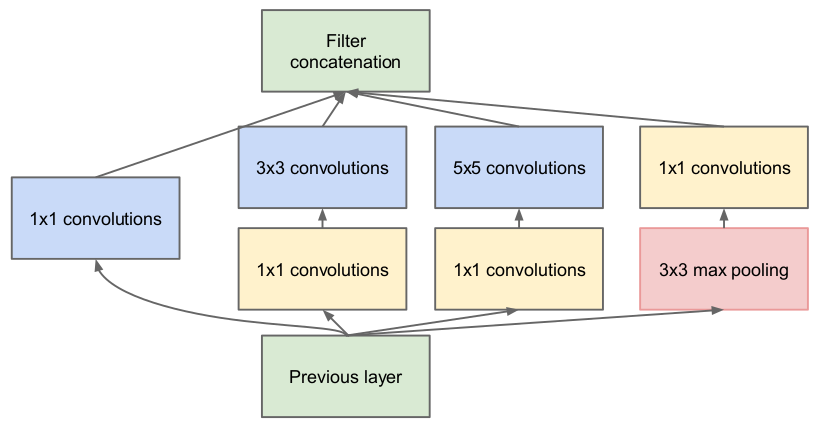
\includegraphics[width=0.5\textwidth]{InceptionModule}
  \caption{Inception module with dimension reduction (taken from \cite{szegedy2015going}).}
  \label{InceptionModule}
\end{figure}

\section{ResNet}
\subsubsection{by Dominique Cheray}
Residual Networks were first presented in 2015 and winner of the ImageNet
Large-Scale Visual Recognition Challenge of the same year. The core idea of
ResNet is the introduction of so-called identity shortcut connections that skip
one or more layers, as shown in figure \ref{ResidualBlock}. A residual block has
two options: either perform a set of functions on the input or skip this step
altogether. \\
The depth of a neural network is of crucial importance for its performance.
However, increasing network depth does not work by simply
stacking layers together. With increasing network depth the accuracy gets saturated
and eventually degrades rapidly and therefore adding more layers to a suitably
deep model leads to higher training error \cite{he2016deep}.
The authors of \cite{he2016deep} argue that stacking layers shouldn't degrade the networks
performance, because one could simply stack identity mappings upon the current
network and the resulting architecture would perform the same. This indicates
that the deeper model should not produce a higher training error than its
shallower counterpart. But optimizing deep networks is difficult and current
solvers cannot find the solution. Therefore they propose a deep residual
learning framework. Instead of hoping each few stacked layers directly fit a
desired underlying mapping they explicitly let these layers fit a residual
mapping. The authors hypothesize that letting the stacked layers fit this
residual mapping is easier than letting them directly fit the desired underlying
mapping. \\
Similar to GoogLeNet several of the residual blocks are stacked upon each other
to construct the final network. It ends with a global average pooling layer
followed by fully connected layer with softmax for the classification. 
\begin{figure}
  \centering
  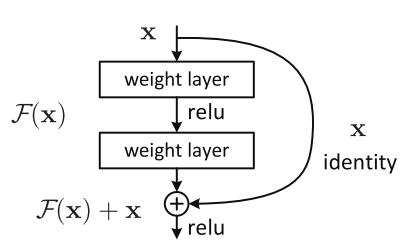
\includegraphics[width=0.4\textwidth]{ResidualBlock}
  \caption{Residual block (taken from \cite{he2016deep}).}
  \label{ResidualBlock}
\end{figure}

\section {Class Activation Mapping}
\label{CAM}
\subsubsection{by Dominique Cheray}
Class Activation Mapping (CAM) is a technique to expose the implicit attention
of Convolutional Neural Networks (CNN) on an image. It highlights the most
informative regions relevant the predicted class \cite{zhou2016learning}. For a
CNN to be used for CAM, its architecture must meet certain requirements. Its
last convolutional layer has to be followed by a layer that performs global
average pooling (GAP) on the convolutional feature maps. The output of the GAP
is then used as features for a fully connected layer that produces the desired
output (categorical or otherwise). \\
The GAP outputs the average of each feature map at the last convolutional layer
and in the fully connected layer a weighted sum of these values is used to
generate the final output. To generate the CAM one now takes the weights of the
fully connected layer belonging to the desired class and the feature maps of the
last convolutional layer and multiplies each feature map by its associated
weight. The weighted feature maps are then added up and upsampled to the size of
the original image. In the resulting image one can identify the image regions
most important to the particular class. Figure \ref{SchematicCAM} shows a
schematic overview of the procedure for generating the class activation maps.
\begin{figure}
  \centering
  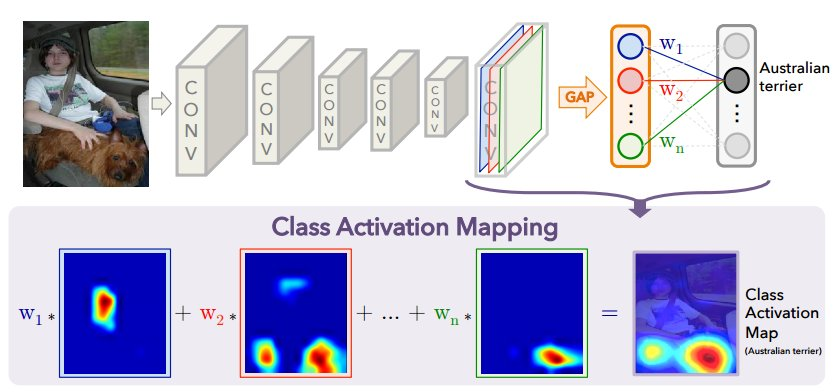
\includegraphics[width=0.9\textwidth]{CAM_graphik}
  \caption{Schematic overview of the procedure for generating the class activation maps (taken from
    \cite{zhou2016learning}).}
  \label{SchematicCAM}
\end{figure}

\section{Data Set}
\label{dataset}
\subsubsection{by Dominique Cheray}
The data set we used in our project is a subset of the MPII Human Pose Dataset
\cite{andriluka20142d}. This data set is a state of the art benchmark for
evaluation of articulated human pose estimation. It includes around
25,000 images and covers 410 human activities. The activities cover a wide range
and span from household activities and leisure activities to sports. Each image
of the data set was extracted from a YouTube video and is provided with an
activity label. In addition the preceding and following unannotated frames are
also provided. \\
For the purpose of this project we concentrated on the sports part of the
data set. In order to keep our data set as large as possible and at the same
time the classes balanced, we have selected the sports that contain the most
pictures and a similar number of pictures. The remaining data set consists of
1576 images distributed over 10 classes. These classes are basketball, horseback
riding, martial arts, paddleball, rock climbing, rope skipping, skateboarding,
softball, tennis, golf. Figure \ref{plotgrid} gives a little insight into the
data set. 
\begin{figure}
  \centering
  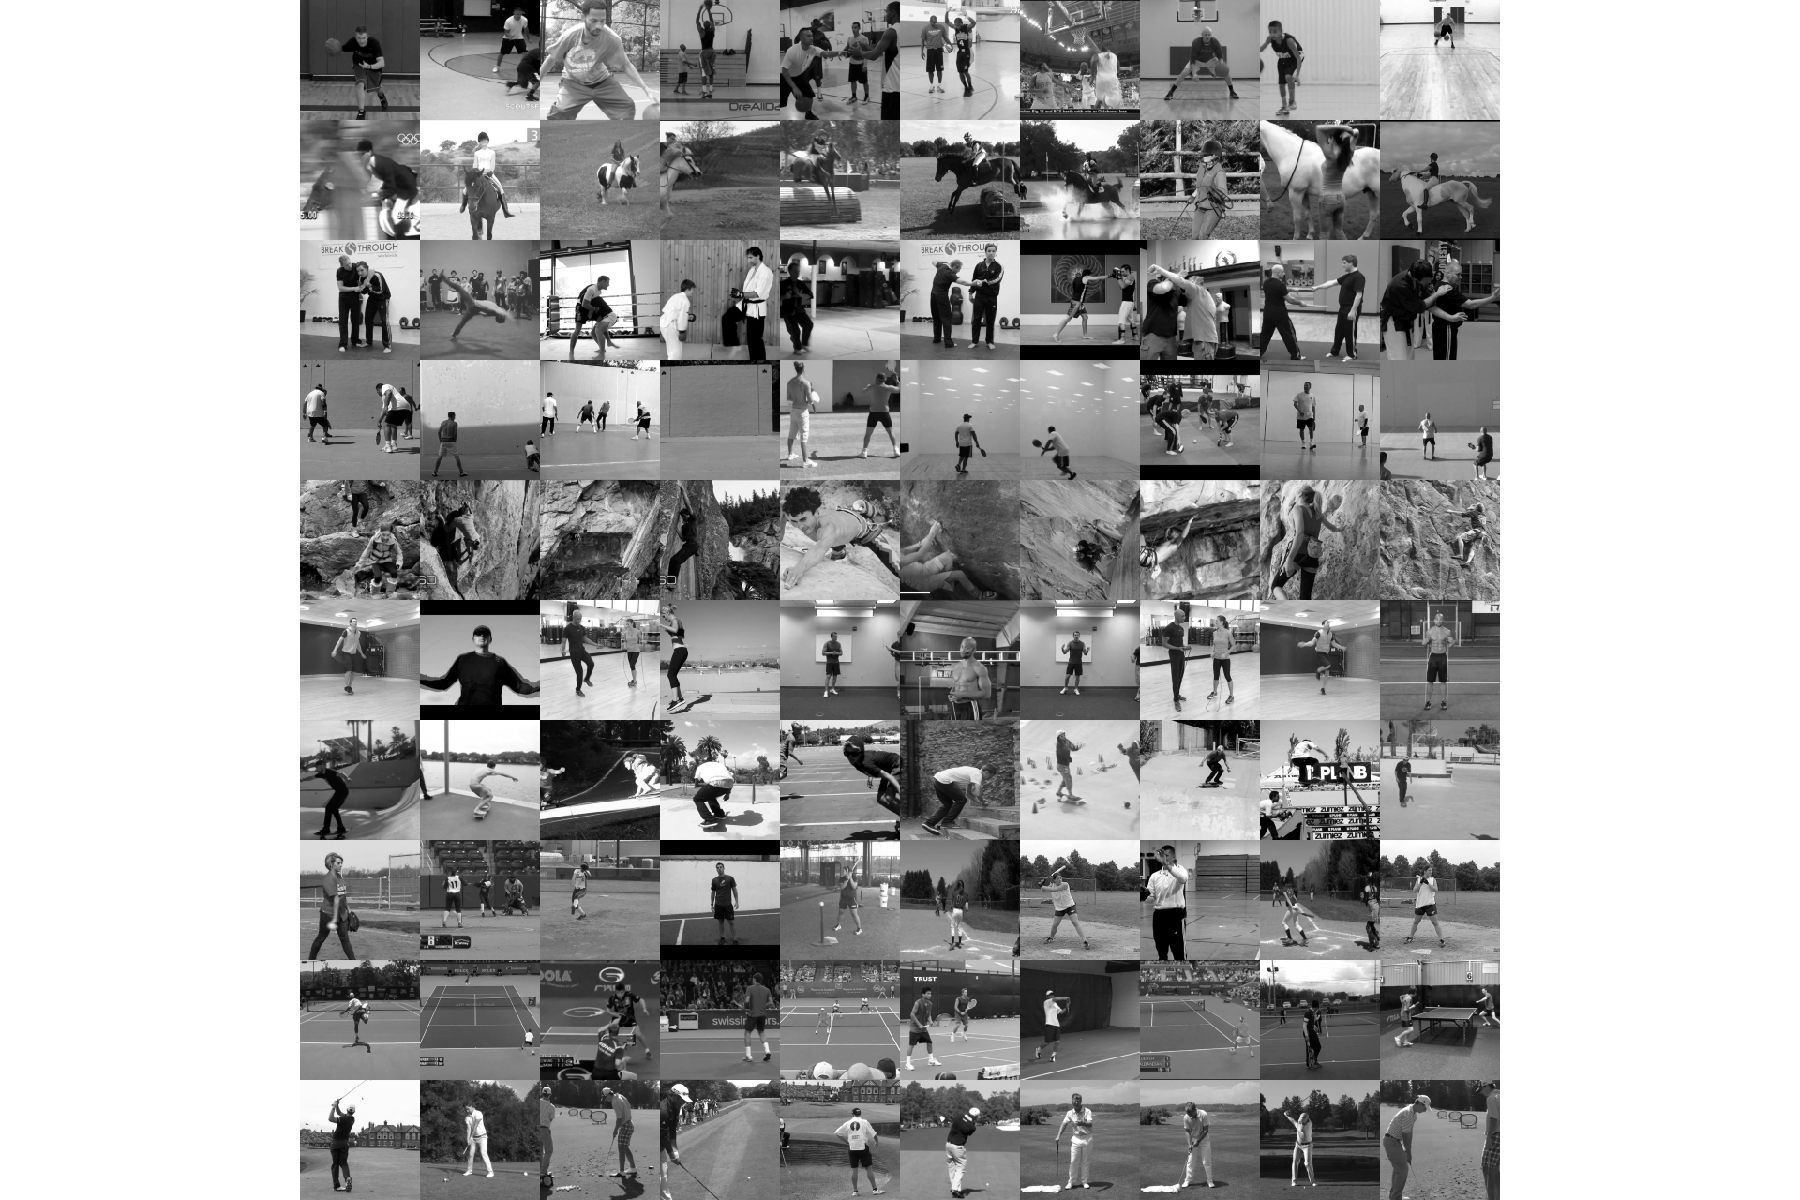
\includegraphics[width=0.6\textwidth]{plotgrid}
  \caption{Samples of the data set - one row is one class.}
  \label{plotgrid}
\end{figure}

\section {Support Vector Machine}
\label{SVM}
\subsubsection{by Manuel Krämer}
The analysis of temporal information can be done by investigating successive frames of a video sequence. We choose, as the method for classification, a Support Vector Machine (SVM) that is suitable because of the comparatively low training effort and a good generalization. \\
In general, the goal of a SVM is to construct a hyperplane in the feature space that separates two classes in a way that maximizes the margin between the two classes. This approach is the reason for the good generalization properties which is better than e.g. the Linear Discriminant Analysis where the margin is not taken into account. The exact behaviour of the margin maximization can be changed with a hyper parameter, often called C-value. This value determines how misclassified points get penalized. If one chooses a high C the model tends to overfitting in order to minimize the training error. A lower C could lead to some mistakes in training but a better generalization, also called soft margin. \\
Since we want to do a multiclass classification the SVM (which is only defined for two classes) uses the so called "one-vs-rest" algorithm. This means that e.g. if you have ten classes you need ten classfiers with class 1 vs all other, class 2 vs all other, etc. These ten classifiers (10 decision surfaces) split the whole feature space into ten separated areas.\\
Another property of the SVM that the kernel-trick ca be used. This means that if you have n-dimensional data the SVM uses a kernel function that computes values in the n+1-dimensional space. This procedure can lead to better results if the data is not linearly separable in n dimension beacuse it maybe is in n+1 dimensions. Often, a radial basis function is used.\\ 
All these aspects make the SVM a good choice for our purpose: It can handle high dimensional data (e.g. images) without a lot of computational effort and it also works well with a small dataset that has only a few instances per class.

\chapter{Methods}
\section{Classification with the Networks}
\subsubsection{by Dominique Cheray}
For the training and testing of the GoogLeNet and the ResNet we randomly
assign 20 \% of the images of each class to the test set and the remaining
images to the training set. Our training set therefore consists of 1266 images
and our test set of 310 images. We train and validate the networks with the
training set and keep the test set for the final testing of the performance
of the networks. \\
Due to the rather small size of our data set we use Data Augmentation to
artificially inflate our data set and avoid overfitting of the networks on the
training data. According to the results of \cite{taylor2017imporving} we apply
a combination of geometric augmentation and cropping since the authors could
show that applying these two methods improved the performance of CNNs
the most. We therefore first resize the training images to 256x256 pixels and
then apply a random transformation to it (either a flip or a rotation).
Afterwards we extract five 224x224 crops from the transformed image, one crop
out of every corner of the image and one out of the center of the image. Later
during training the prediction of the network is averaged over these five crops
to get one prediction for the underlying original image. \\


\section{Temporal Analysis with SVM}
\subsubsection{by Manuel Krämer}
The approach we used to investigate the temporal information in image sequences (videos) and compare it to a static method like the single frame neural network classification is the following:

\begin{enumerate} 
\item Choose 3,5,7 or 9 successive frames of a video sequence with a spacing of 5 frames (Since the videos aren't that long; if we choose 9 frames we needed to decrease the spacing to 4)
\item Process each single frame through the GoogLeNet and extract the features from the last hidden layer (which is a feature vector of size 1024)
\item Concatenate all the feature vectors to a single image sequence feature vector
\item Do the classification of these image sequence feature vectors with one of the ten labels (see ch. \ref{dataset}) with a SVM
\end{enumerate}

The described algorithm is shown in fig. \ref{fig_svm}.

\begin{figure}
  \centering
  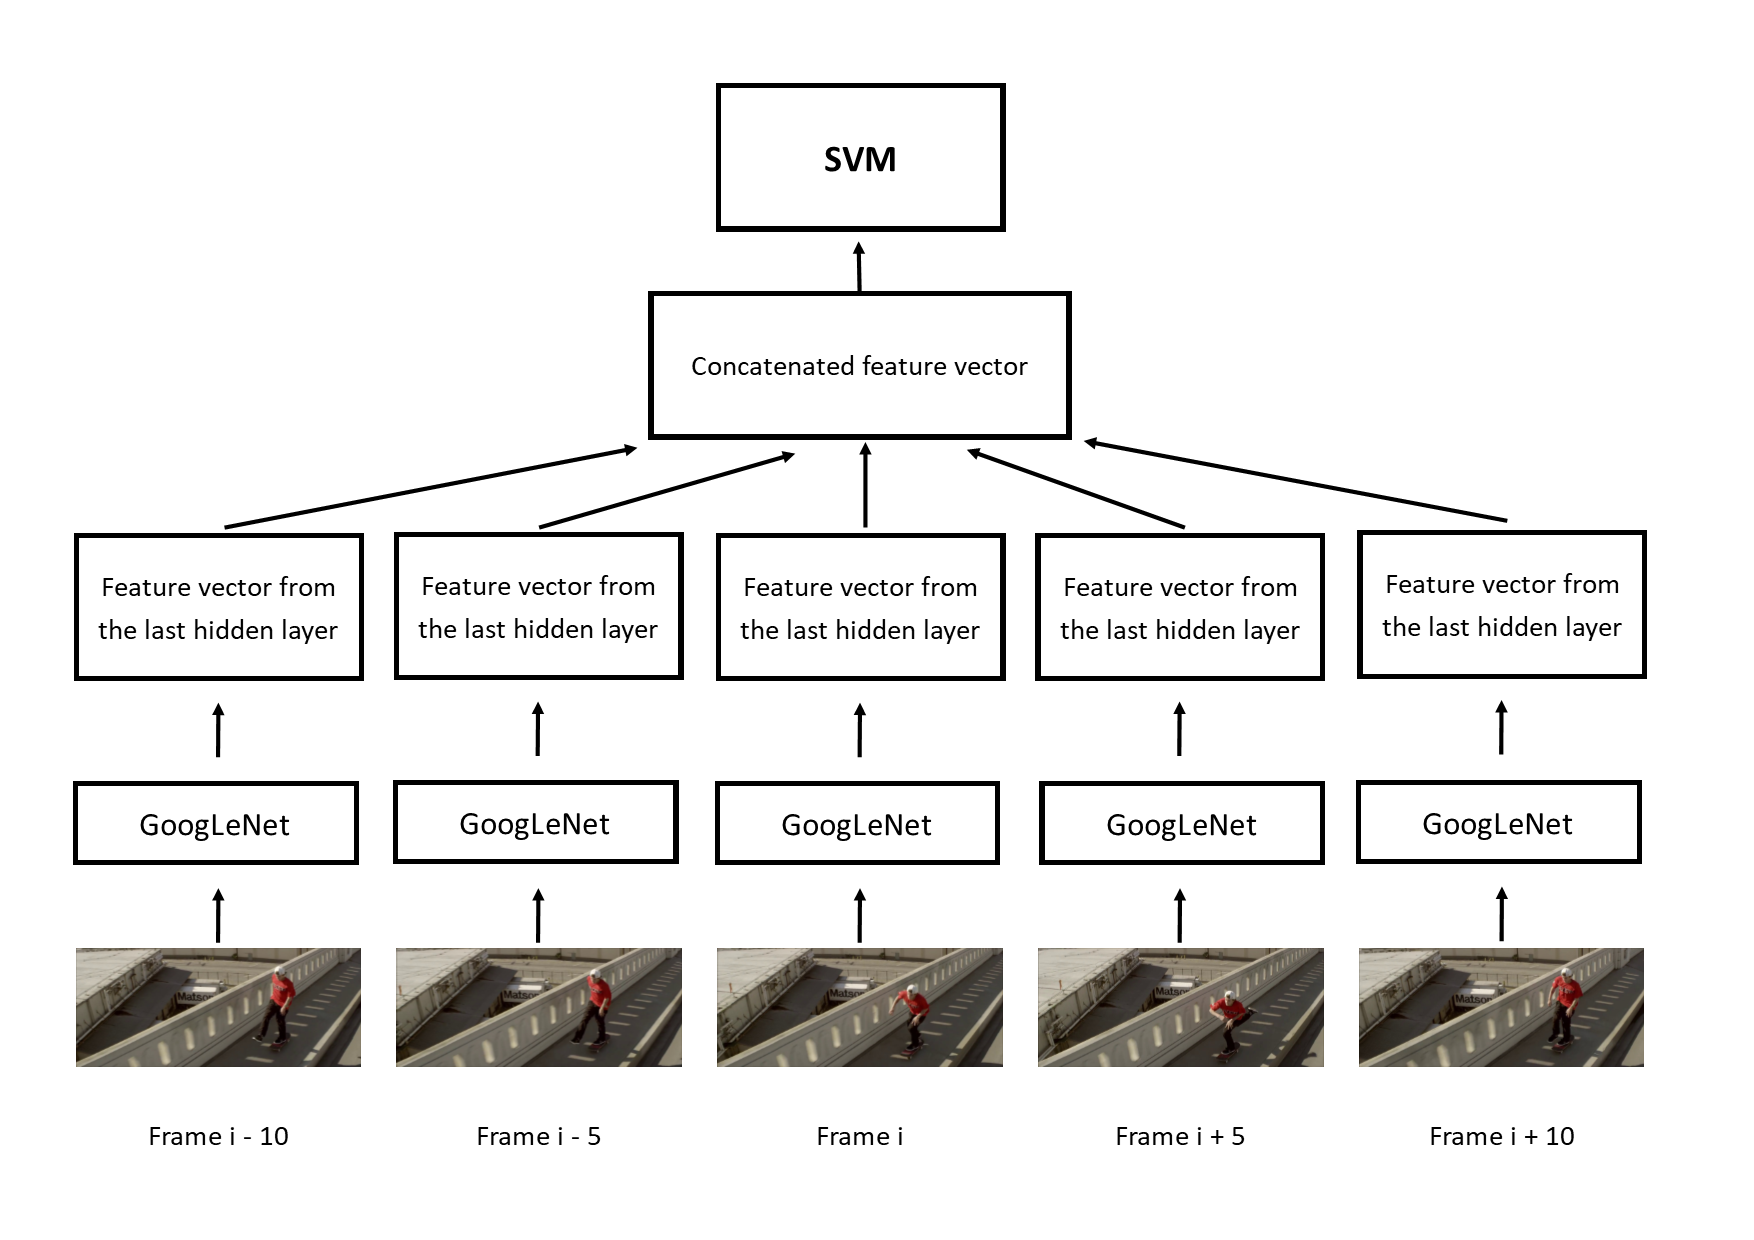
\includegraphics[width=0.7\textwidth]{Illustration_SVM.png}
  \caption{Algorithm of the temporal analysis using a SVM. Here you can see one example of a video sequence of 5 frames}
  \label{fig_svm}
\end{figure}

The Classification with the SVM can be done with several possibilities as you can see in ch. \ref{SVM}. The best results were achieved by a linear SVM (linear kernel), a C-value of 1 and the "one-vs-rest" algorithm. 


\chapter{Methods}
\section{Classification with the Networks}
\subsubsection{by Dominique Cheray}

\section{Temporal Analysis with SVM}
\subsubsection{by Manuel Krämer}
Our results are shown in table \ref{result_table_SMV} and fig. \ref{result_fig_svm}.
One can see that more temporal information (more frames) lead to an increasing accuracy in training. The testing dataset shows the same behaviour besides the fact that at 9 frames it is decreasing compared to 7 frames. \\


\begin{table}[]
\centering
\begin{tabular}{|l|l|l|}
\hline
3 frames with spacing 5 & 77.6\% & 47.4\% \\ \hline
5 frames with spacing 5 & 88.9\% & 48.4\% \\ \hline
7 frames with spacing 5 & 95.2\% & 52.6\% \\ \hline
9 frames with spacing 4 & 97.3\% & 50.3\% \\ \hline
\end{tabular}
\caption{Classification accuracy of the SVM for 3,5,7 and 9 successive frames of a video sequence}
\label{result_table_SMV}
\end{table}

\begin{figure}
  \centering
  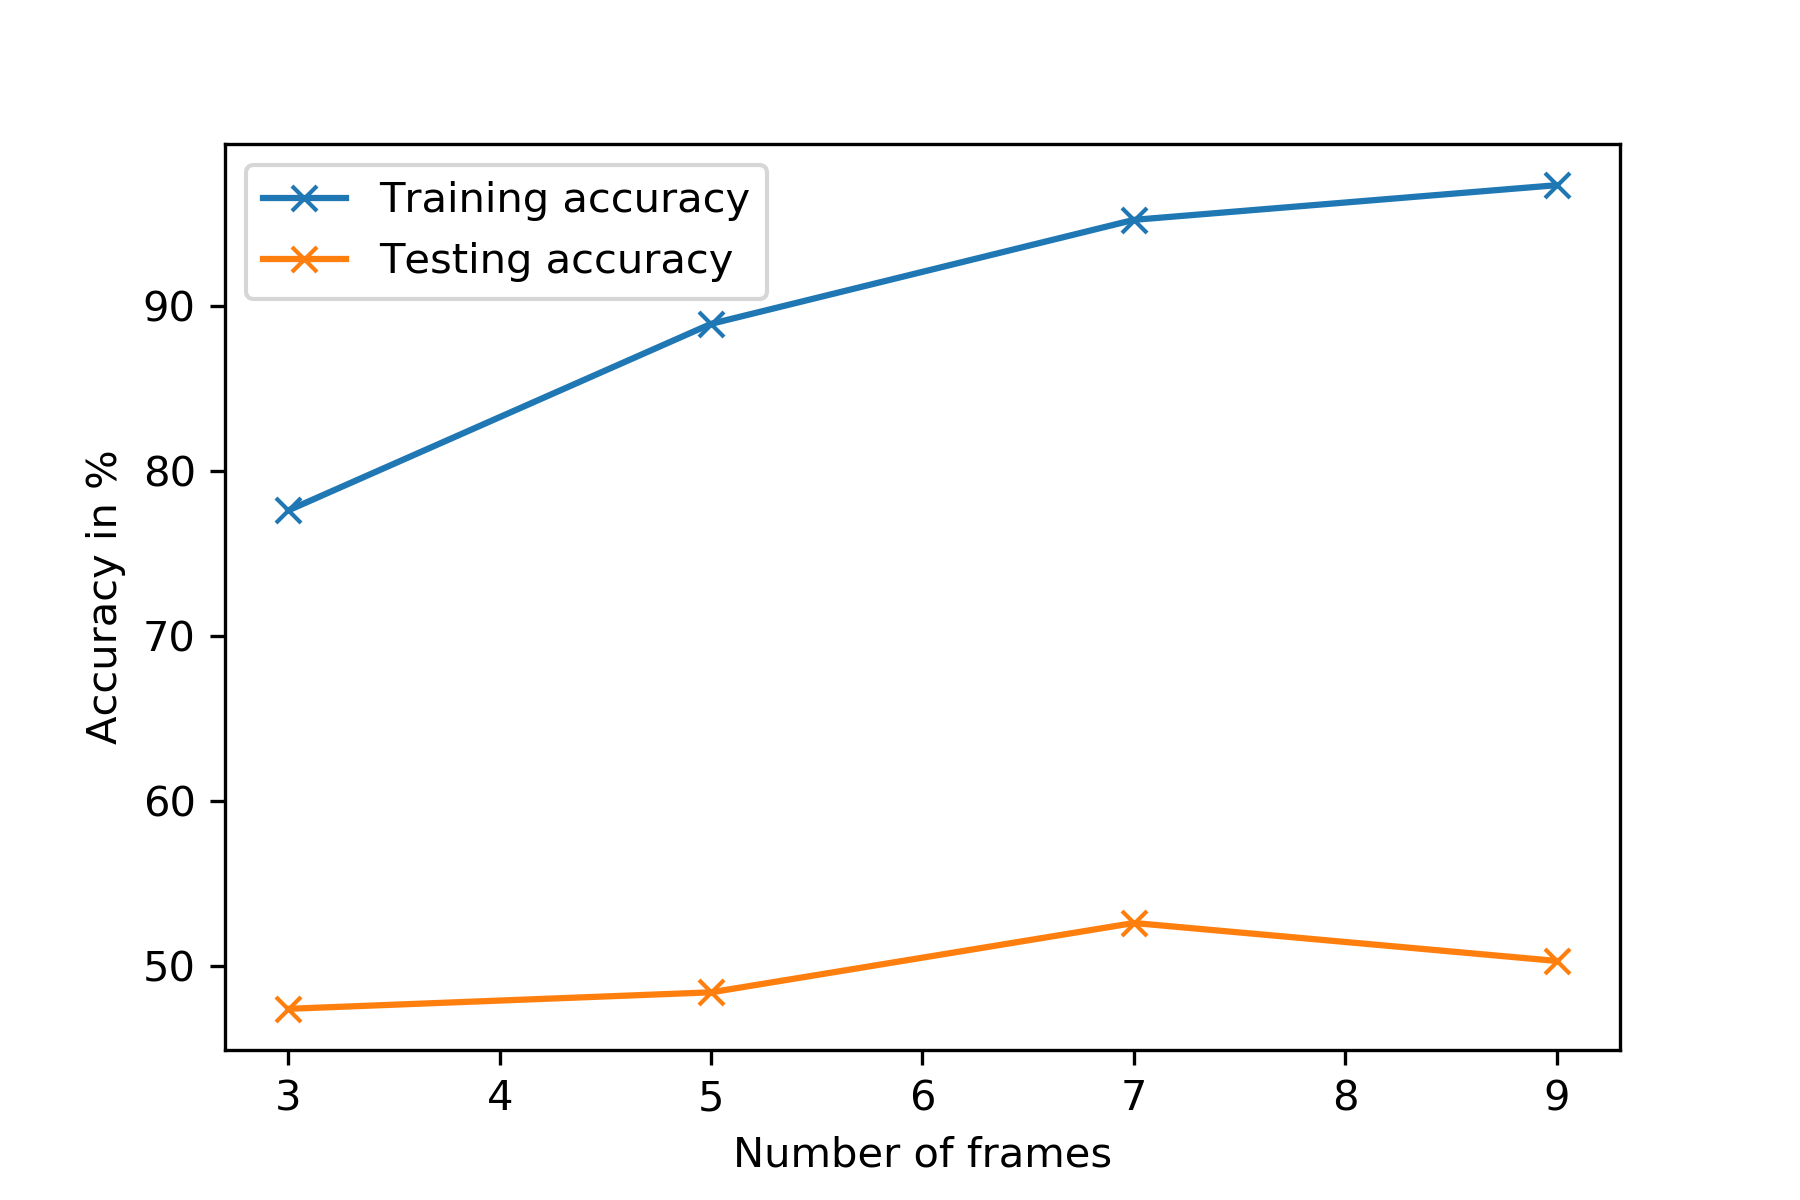
\includegraphics[width=0.7\textwidth]{AccuracySVM.png}
  \caption{Accuracy of the SVM vs. number of images considered for classfication}
  \label{result_fig_svm}
\end{figure}


\bibliography{literature}

\end{document}
